\dictum[Antisthenis]{There is no horse, there is horses}

\begin{summary}
\item \emph{Antisthenis} is a system for incremental evaluation of
  algebraic expressions using heuristics to optimize the order in
  which subexpressions are evaluated and to calculate some classes of
  self referrential computations.
\item Mealy arrows are a construct to implement adaptable computations
  that can can prodice a value and a new, semantically equivalent
  computation. Each iteration adapts to the previous caching values
  and changing the evaluation plan to be more efficient.
\item Antisthenis computations are implemented as network of mealy
  arrows that compose larger adaptive (incremental and partial)
  computations.
\item Machines are named processes that can be referred to by other
  machines. Antisthenis can handle some classes of self referrential
  computations.
\item We implement antisthenis operations to cover requirements of the
  FluiDB physical planner:

  \begin{itemize}
  \item calculate min/sum of natural numbers -- used to compute cost
  \item boolean functions -- used determine node materializability
  \item calculate min/sum of numbers annotated with certainty metrics
    -- used to calculate the cost of materialization of nodes give
    nodes that \emph{might} be magterialized.
  \end{itemize}
\end{summary}

This chapter goes in depth descibing the various parts that compose
Antisthenis, a system we developed to assist the FluiDB planner in
incrementally and efficiently computing costs and checking if nodes in
the QDAG are materializable during the evolution of the inventory.

The chapter starts with an introduction about the motivation for
developing Antisthenis as a collection of synchronously communicating
processes performing incremental computation. Next we look at some
background concepts most of which relate to notions for computation
and our conception of a Mealy arrow that builds on those notions to
enable the construction of Antisthenis processes. In the following
section we describe the core of Antisthenis, which is the internal
construction of a single antisthenis process. From there we move on to
describe some specific operation implementations that are useful for
FluiDB and then describe the systems that facilitate
intercommunication and high level organization of Antisthenis
processes. Finally, we conclude with some shortcomings and some future
future work that can be done to make Antisthenis easier to apply to
solutions other than FluiDB.

\section{Introduction}
\label{sec:antisthenis_intro}

The order in which an expression is evaluated can be important not
only for the performance of the expression evaluation but, in the
context of infinite expressions, for the very termination of the
evalution itself.

Expressions are typically modelled as abstract syntax trees or
computation graphs, and evaluation is commonly modelled as a reduction
of that tree or DAG. Depending on the evaluation strategy each operand
is either fully or partially evaluated. Typically, the strategy for
evaluating the subexpression operand however is oblivious to the
parent expression and a partially evaluated subexpression (thunk) is
opaque from the perspective of the parent expression. Breaking this
assumption provides some opportunities for incremental computation and
efficient evalaution in the presence of non-total arguments.

We built \emph{Antisthenis} around this principle to achieve three
important goals:

\begin{itemize}
\item Incrementally evaluate an expression, i.e. to only re-evaluate
  the parts of it that depend on parameters that were updated with
  respect to the last time the expression was evaluated.
\item Take advantage of absorbing elements and other operator-specific
  strategies for early stopping the evaluation.
\item Often sub-expressions are not total, i.e. they may not be
  computable. A common reason for that is the expression being
  self-referential. These errors may be detrimental to the evaluation
  the top level expression, but often as we will see they are not.
\end{itemize}

Incremental computation is a tool for efficiently evaluating
expressions of variables that change over time. The area has received
some attention recently
\cite{bhatotiaIncoopMapReduceIncremental2011,hammerAdaptonComposableDemanddriven2014a}. An
incremental evaluator will typically accept a directed acyclic graph
(DAG) of interdependent computations like the following one

\begin{align*}
A &= a + B + C + D  \\
B &= C \times b \\
C & = D + c \\
D &= 0
\end{align*}

Which can be represented as a dag in figure
\ref{fig:example_antisthenis_dag}.

\begin{figure}[H]
\centering
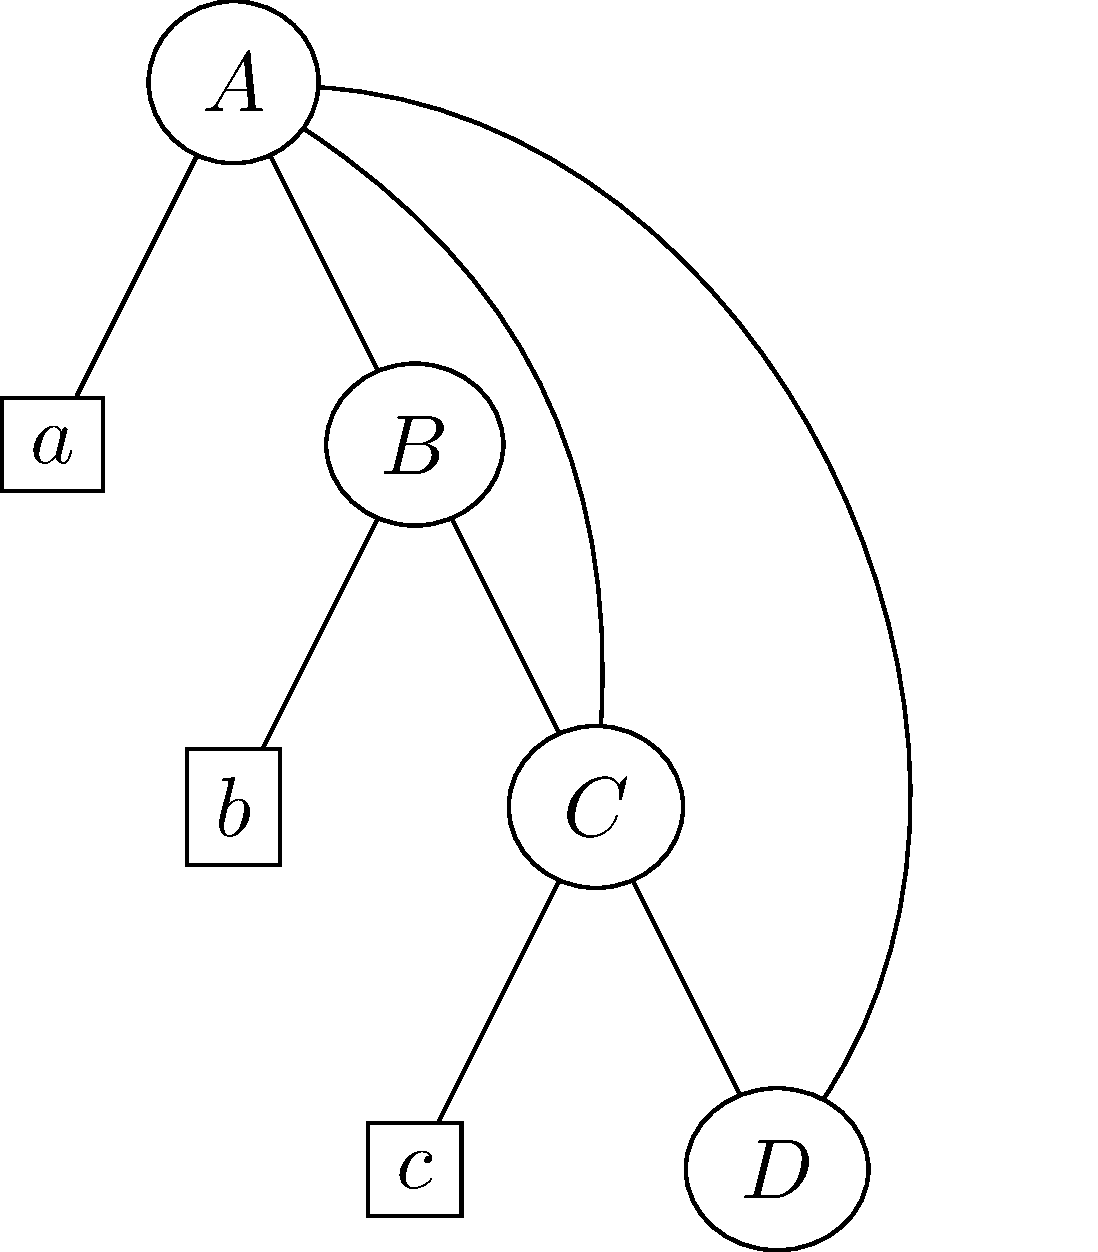
\includegraphics[width=.5\textwidth]{./imgs/example_antisthenis_dag.pdf}
\caption{\label{fig:example_antisthenis_dag}A computation DAG.}
\end{figure}

Where \(A\), \(B\), \(C\), and \(D\) are expression nodes in the DAG
and \(a\), \(b\), and \(c\) are parameters that change over
time. \(A\) depends on all three parameters. A non-incremental
evaluation system would evaluate all four nodes every time a value
were requested, regardless of whether and which parameters have
changed. Incremental evalutaion systems keep track of which variables
change and only re-evaluate the nodes of the DAG that have been
updated. In our example if only the parameter \(b\) has been updated
since the last time \(A\) was evaluated, in the meantime only \(A\)
and \(B\) would need to be re-evaluated.

Incremental evaluation systems employ a wide range of tricks from
simply memoizing the functions
\cite{pughIncrementalComputationFunction1989} to more complex
strategies like \cite{hammerAdaptonComposableDemanddriven2014a} where
changes in parameters are propagated in the form of dirtying DAG nodes
and more explicitly breaking the computation into reusable parts.

To our knowledge none of the existing approaches to incremental
computation take into account the presence of either absorbing
elements or non-compuatable subtrees (i.e. recursive values) in their
scheduling the evaluation order. It is either done naively or left up
to the programmer. However, it is a hard requirement of the FluiDB
query planner for the incremental computing framework to automatically
exploit the properties of the computation at hand in order to
incrementally compute node materializability and query costs in the
presence of different materialized query sets. Furthermore, in all the
approaches we are aware of the network of sub-expressions was assumed
to be well-behaved, in that all nodes return a valid value and there
are no cyclical references.

The main principle behind the architecture of Antisthenis is to
manipulate the order in which sub-expressions are evaluated in order
to exploit properties of the parent operator to avoid fully evaluating
each of the sub-terms. For example when evaluating the cost of a
database query we take the result of the computation is the minimum
cost of each of the possible logical plans. It is unlikely that one
would need to come up with a full estimation of each plan, especially
the more expensive ones, before realising the lowest cost. Instead, we
would like to accumulate a lower bound for the cost of each plan.

Another prime example of an opportunity pruning the expression tree is
the exploitation of absorbing elements. In the general case, in a
non-lazy evaluation strategy, to compute the value of a function
\(f(A,B,C)\) where \(A\), \(B\) and \(C\) are expressions, we would
need to fully evaluate \emph{all} three arguments first. Since the
absorbing element of multiplication in the reals is 0, for
\(f(a,b,c) := a \times b \times c\), a result of 0 for the first
argument \(A\) would render the evaluation of the rest of the
arguments futile.

As alluded to, a lazy evaluation strategy paired with a Sufficiently
Advanced Compiler, can take steps towards mitigating this
problem. This can only go so far, however. Consider the following
example:

\begin{align*}
A &= B \times C \times D \\
B &= \sum_i{i} \\
C &= 0 \\
D &= \sum_i{i}
\end{align*}

Here, when evaluating \(A\), a traditional evaluation system would
look at the first argument first, namely \(B\). \(B\) is very
expensive to evaluate and very soon a human would figure out that it
will never evaluate to zero. \(C\), however, does evaluate to zero,
and once that is evaluated the evaluation of \(A\) is complete. In a
complex set of automatically generated such expressions it is
important that the evaluator does not fall into a deep expression when
a very shallow one could yield an absorbing value.

Early stopping a computation is not useful only to avoid extra
work. As we mentioned, many incremental computation systems assume
that all sub-computations terminate successfully. Due to the presence
of cycles in FluiDB graphs we need to take seriously the case where a
sub-expression will fail to terminate. In this case the parent
expression needs to exhaust all possibilities that could lead to a
value.

\begin{align*}
A &= min(B, C, D) \\
B &= b_1 + b_2 \cdot D \\
C &= c_1 + c_2 \cdot A \\
D &= d_1 + d_2 \cdot B \\
b_1 &= b_2 = d_1 = d_2 = 1 \\
c_1 &= 3 \\
c_2 &= 0
\end{align*}

Here \(B\) and \(D\) are clearly not computable but in the context
where these values represent cost of evaluations for nodes \(A\)
should evaluate to 3 and \(A\) should evaluate to \(C =
3\). Furthermore, \(A\) should depend \emph{all} parameters for the
validity of its value while \(C\) should depend only on \(c_1\) and
\(c_2\).


\section{Background}

In order to describe our model of self-adjusting computation we need
to lay the groundwork by describing the basic model of computation as
understood by ML like languages, and specifically Haskell. These
languages define computations as first class values that have
parametric types. A computation of type \hask{f a} can be understood
as a computation that when executed would generate a value of type
\hask{a}. In that sense \hask{f} is a generic type with one type
parameter \hask{a}, thereby being of kind \hask{* -> *}, whereas
\hask{a} and \hask{f a} are both of kind \hask{*}. For example,
in Haskell, we represent as \hask{IO Int} the type of a computation
that interacts with the outside world in order to compute an integer,
e.g. by reading user input, by writing files, or, as the meme in the
community goes, by launching missiles.

From the perspective of a programming language in order to manipulate
computation it is useful to be able to change computations, i.e. to be
able to create morphisms \hask{f a -> f b} from simpler primitives in the
language. The notation of a the arrow \hask{->} used here is a function
within the basic framework of the language, a simple mapping between a
value of type \hask{f a} to a value of type \hask{f b}. This is indeed already
computation carried out by the runtime.  In that sense it is
\emph{implicit} computation. We have little control over the
conditions under which it is carried out, especially in a lazy
language like haskell, and we consider it to be pure, with no
effects. This will become important when we discuss arrows and
profunctors.

Returning to our higher kinded (of kind \hask{* -> *}), explicit
computations, commonly in haskell a hierarchy of 3 typeclasses
(interfaces) that computations conform to has been established, each
of which provides a different way of producing morphisms of the
computation itself, and therefore each of which allowing different
computations to be expressed by type \hask{f}. While these typeclasses are
more general than refering only to computations, we will try to
provide an intuition of each for them in reference to computations, to
avoid overwhelming the reader with the full generality of these
constructs. The reader is encouraged to notice how the weaker, more
general, typeclasses presented first, more intuitively describe
containers of values and as we strengthen the constraints and require
more operations of our objects it becomes harder to think of
containers that fit the constraints and notions of the values as
computations becomes more natural.

\subsection{Functor}

For computations implementing the \hask{Functor} typeclass we can
create a morphism of the computation from a normal haskell
function. For every functor \hask{f} then, there must be a function
\hask{fmap :: (a -> b) -> f a -> f b} that abides by the functor (see
listing \ref{lst:functor_def})
\cite{mcbrideApplicativeProgrammingEffects2008}. In plain english,
given a computation and a function that can transform the result of
the computation we can get a new computation that is equivalent to the
original computation but yielding the transformed result. The functor
laws (see listing \ref{lst:functor_laws}), which all valid
implementations of a functor must follow, assert that applying the
identity function to the result of a computation does not change the
computation itself and that \hask{fmap} ing has no other effect on the
computation other than changing its result.
\begin{code}
\begin{haskellcode}
class Functor f where
  fmap :: (a -> b) -> f a -> f b
\end{haskellcode}
\caption{\label{lst:functor_def}The functor inteface in haskell.}
\end{code}

It is common to understand functors in the context of haskell as
mappable containers that can hold any type value. One could think of a
computation that supports the functor interface as a computation that
results in a functorial container. An example of a computation that is
\emph{not} a functor might be one that produces a set of values,
because a set of values requires that the values are comparable, and
not all per element value transformations of a set are valid. For
example a set of integers \hask{Set Int} can be unambiguous for the
language but a set of functions \hask{Set (Int -> String)} is not
unless we define a notion of equality for functions.

\begin{code}
\begin{haskellcode}
-- Identity
fmap id == id
-- Composition
fmap (f . g) == fmap f . fmap g
\end{haskellcode}
\caption{\label{lst:functor_laws}Laws that any valud functor inteface interface must obay.}
\end{code}


\subsection{Applicative}

Computations that are applicative
\cite{mcbrideApplicativeProgrammingEffects2008} functors are
computations that can be combined in "no particular order". In
particular an applicative functor must implement \hask{ap :: f (a ->
  b) -> f a -> f b} (more commonly written as \hask{<*>} which is a
bit harder to pronounce) and \hask{pure :: a -> f a} (see listing
\ref{lst:applicative_def}). Applicatives are more often described in
terms of computation than functors. Firstly, this means that we must
be able to construct a trivial computation that just returns a given
value, meaning that there must be no restriction on the kinds of
values an applicative computation can yield. For example a computation
that yields only integers is not an applicative because then there
would no way to universally quantify the argument of
\hask{pure}. Incidentally it is not a functor either for the same
reason, namely that we wouldn't be able to universally quantify the
output of the input function of \hask{fmap}.

\begin{code}
\begin{haskellcode}
class Functor f => Applicative f  where
  (<*>) :: f (a -> b) -> f a -> f b
  pure :: a -> f a
\end{haskellcode}
\caption{\label{lst:applicative_def}The interface of a haskell applicative functor.}
\end{code}

Furthermore, from the definition of \hask{ap} or \hask{<*>} we
understand that two computations that are applicative functors can be
combined into one computation with no restriction on the order thtat
they are evaluated. There are a few examples of applicatives being
used to represent parallelizable computation, the most prominent of
which being Facebook's Haxl \cite{marlowHaxlProjectFacebook2013}

Like with \hask{Functor} the interface of applicative must be subject
to the applicative laws presented in
\ref{lst:applicative_laws}. Essentially these formalize the triviality
of \hask{pure}.

\begin{code}
\begin{haskellcode}
-- Identity
pure id <*> v = v
-- Composition
pure (.) <*> u <*> v <*> w = u <*> (v <*> w)
-- Homomorphism
pure f <*> pure x = pure (f x)
-- Interchange
u <*> pure y = pure ($ y) <*> u
\end{haskellcode}
  \caption{\label{lst:applicative_laws}Laws that any valid applicative
    intreface must obay}
\end{code}

\subsection{Monad}

A meme in the functional community defines monads as "monoids in the
category of endofunctors". To the unfamiliar reader this may take a
second to parse, but it is really just a fancy way of saying something
fairly simple: we can transform any nested monadic functor \hask{f (f
  a)} into a flat one \hask{f a}, and if the stack is large \hask{f (f
  (... f (f a)))} the order in which the functors are collapsed does
not matter. In the context of computations this implies that nested
computations run from inside out, the inner computation is run first
and then the outer one is run. The "and then" part is what a monad is
meant to bring to the table. Viewed as computations monads must have
all the properties of functors and applicatives but they must also
implement the operation \hask{(>>=) :: f a -> (a -> f b) -> f b} where
\hask{>>=} is pronounced \hask{bind}. The computation described by the
first argument of \hask{>>=} must be executed \textbf{first} in order
to generate the argument for the function in the second argument which
must \textbf{then} produce the result. We commonly represent a monadic
functor by the characer \hask{m} rather than the character \hask{f}
that we used for functors and applicatives. Monads are the most
commonly used abstraction to describe computations comprised of
interdependent steps. The haskell interface for monads is succinctly
presented in listing \ref{lst:monad_def}

\begin{code}
\begin{haskellcode}
class Applicative m => Monad m where
  return :: a -> m a
  (>>=) :: m a -> (a -> m b) -> m b
\end{haskellcode}
  \caption{\label{lst:monad_def}Definition of the interface of a
    haskell monad.}
\end{code}

Monad implementations need to adhare to laws laid out in listing
\ref{lst:monad_laws}. These laws are similar to the applicative laws
in that they formalize the trivality of \hask{pure}, now called
\hask{return}, in relation to the \hask{bind} operator this
time. However, unlike the applicative laws, monadic laws introduce the
law of associativity that may seem strange to a reader unfamiliar with
Kleisli arrows \cite{dawsonCompoundMonadsKleisli2007}. The essence of
the monad, when focusing on the second argument of bind (the one typed
\hask{a -> m b}), and which is codified by the monad laws is that a
monad \hask{m} must give rise to a category, referred to in the
literature as the Kl category.

A category needs a set of objects and a domain of arrows that can be
composed. Further we need the arrow composition to be associative and
an identity arrow that maps objects to themselves. An obvious category
is formed by all objects in haskell, haskell functions as arrows and
\hask{id :: a -> a} as the identity arrow. This is commonly referred to as
the hask category. As aluded to earlier, this category does describe
computation albeit in a more implicit manner. The monad laws assert
that each monad gives rise to a kleisly category where objects are the
objects of hask, arrows \hask{a \textasciitilde{}> b == a -> m b} and the identity arrow is
\hask{return}. Moving forward we will see how, capitalizing on this
conception we can come up with a more flexible/

\begin{code}
\begin{haskellcode}
-- Left identity
return a >>= k = k a
-- Right identity
m >>= return = m
-- Associativity
m >>= (\x -> k x >>= h) = (m >>= k) >>= h
\end{haskellcode}
  \caption{\label{lst:monad_laws}Laws that any valid monad
    implementation must abide \cite{yorgeyTypeclassopedia2009}.}
\end{code}

\subsubsection{Monad examples}

To make the concept tangible we provide a few examples of how monads
encapsulate computational effects by looking at four monads: \hask{Maybe},
\hask{State} , \hask{IO}, and \hask{Free}.

\paragraph{Maybe}

The \hask{Maybe} functor (defined in listing \ref{lst:maybe_def})
implments partiality. In other languages the same concept may be
called \hask{opt} or \hask{Option}. A partial function is denoted
\hask{a -> Maybe b} because it may return a value or not return a
value.

\begin{code}
\begin{haskellcode}
data Maybe a = Just a | Nothing
\end{haskellcode}
  \caption{\label{lst:maybe_def}Definition of the \hask{Maybe} monad.}
\end{code}

Composability of the Kleisli arrow allows us to compose multiple
partial functions into new ones, thus creating computations that can
trivially fail. \hask{Maybe} provides a good opportunity to
distinguish between \hask{Applicative} and \hask{Monad}. Considering
the two programs in listing \ref{lst:maybe_example} where we only care
about \hask{Maybe} as an \hask{Applicative}. The semantics of the
program do not specify whether calling \hask{invAdd} will cause
\hask{inverse a} or \hask{inverse b} to be computed first or if they
will be computed in parallel. No order is imposed between
them. However, in the program presented in \ref{lst:maybe_example2}
when evaluating the function \hask{f} the expression \hask{inverse a}
\textbf{must} be evaluated before the \hask{toInt} so that
\hask{toInt} has an input to operate on.

\begin{code}
\begin{haskellcode}
inverse :: Double -> Maybe Double
inverse a = if a == 0 then Nothing else Just (1 / a)

invAdd :: Double -> Double -> Maybe Double
invAdd a b = (+) <$> inverse a <*> inverse b
\end{haskellcode}
  \caption{\label{lst:maybe_example}Example usage of the \hask{Maybe}
    applicative functor.}
\end{code}

\begin{code}
\begin{haskellcode}
inverse :: Double -> Maybe Double
inverse a = if a == 0 then Nothing else Just (1 / a)

toInt :: Double -> Maybe Int
toInt a =
  if a == fromInteger (round a)
    then Just (round a)
    else Nothing

f :: Double -> Maybe Int
f a = inverse a >>= toInt
\end{haskellcode}
\caption{\label{lst:maybe_example2}Example usage of the \hask{Maybe} monad functor.}
\end{code}

\paragraph{State}

A \hask{State} monad (listing \ref{lst:state_monad_def}) encapsulates
a computation that depends on mutable state of type \hask{s}.

\begin{code}
\begin{haskellcode}
newtype State s a = State (s -> (a,s))
\end{haskellcode}

  \caption{\label{lst:state_monad_def}The state monad describes
    mutable state.}
\end{code}

\hask{State} is essentially a function that accepts some state, modifies it
and returns it along with a value. In C-like languages the operator to
compose different components that operate on the and local state is
\cpp{;}. \cpp{f() ; g() ;} means that \hask{f()} can have arbitrary side effects on
the global state and must be computed entirely before \hask{g()}. In our
slightly more precise flavor of effectful computations \hask{f >> g} as a
\hask{State} composes a state functor that expects some state value, passes
it to \hask{f} which modifies it and passes it to \hask{g}.

\paragraph{IO}

The \hask{IO a} monad is "magical" in the sense that it is completely
opaque to the runtime. It represents the interaction of our haskell
program with the outside world, and since all haskell functions are
pure haskell can be thought of as metalanguage that defines programs
composed of different \hask{IO a} components called the \hask{main ::
  IO ()}. The components of an \hask{IO} computation are guaranteed to
be evaluated one after the other.

This is demonstrated in \ref{lst:io_naive_example}. Because monads are so
ubiquitous haskell provides some syntactic sugar called the \hask{do}
notation. The same program is presented in a much more readable for in
\ref{lst:io_sugar_example}.

The functions \hask{putStrLn :: String -> IO ()} takes a string and returns
a computation that would show the string on stdout. \hask{getLine :: IO
String} is a computation that reads a line from stdin and retains its
value. The \hask{main :: IO ()} is a special variable that a haskell
program needs to define, all the haskell runtime essentially does is
run the IO computation that \hask{main} refers to.

\begin{code}
\begin{haskellcode}
main :: IO ()
main = putStrLn "What's your name?"
       >> getLine
       >>= (\name -> putStrLn ("Hello " ++ name))
\end{haskellcode}
  \caption{\label{lst:io_naive_example}Sequanecing IO interactions
    using the \hask{IO} monad.}
\end{code}

\begin{code}
\begin{haskellcode}
main :: IO ()
main = do
  putStrLn "What's your name?"
  name <- getLine
  putStrLn ("Hello " ++ name)
\end{haskellcode}
  \caption{\label{lst:io_sugar_example}Sequanecing IO interactions
    using the \hask{IO} monad also using the \hask{do} notation.}
\end{code}

\paragraph{Free monad}

The free monad is slightly more convoluted than the ones we talked
about so far. Without getting to deep into what free structures are in
generalk (\cite{bartoszmilewskiDaoFunctionalProgramming} is a
recommended source), a free monad is a structure that only supports
the monad interface in a law-abiding way. The only difference is that
instead of focusing on the \hask{>>=} operator that we saw so far, it
instead has a constructor corresponding to the equivalent operator
\hask{join} presented in listing \ref{lst:join_monad_op}.

\begin{code}
\begin{haskellcode}
join :: Monad m => m (m a) -> m a
join m = m >>= id

-- and also
(>>=) :: Monad m => m a -> (a -> m b) -> m b
m >>= f = join (fmap f m)
\end{haskellcode}

  \caption{\label{lst:join_monad_op}The bind (\hask{>>=}) and join
    operations on a monad are equivalent given that monads are also
    functors.}
\end{code}

A free monad \hask{Free f m} then is equivalent to the \emph{functor}
\hask{f} that is stacked on top of itself zero or more times \hask{f
  (f ( ... f (f a)))}. It essentially turns a functor into a monad for
"free" -- as long as you don't mind that it actually a stack of nested
functor rather than a single layer like monads are. Listing
\ref{lst:free_def_naive} presents a simple implementation, although
the implemetation in \ref{lst:free_def} is more common. Free monads
are particularly important for our implementation of antisthenis.

\begin{code}
\begin{haskellcode}
data Free f a
  = Pure a
  | Free (f (Free f a))
\end{haskellcode}
  \caption{\label{lst:free_def_naive}A simple implementation of the free
    monad type.}
\end{code}

\begin{code}
\begin{haskellcode}
newtype FreeF f a x = Pure a | Free (f x)
data FreeT f m a = m (FreeF f a (FreeT f m a))
\end{haskellcode}
  \caption{\label{lst:free_def}A simple implementation of the free
    monad type.}
\end{code}

\subsection{Arrows and profunctors}

So far we constructed our objects depending on an underlying category
(Hask) provided by the programming language to get a basic notion of
arrows that represent pure functions. This is a very opaque and
inflexible kind of computation but a strong base on which to build
ones better suited to our needs. In this subsection we will look at a
generalization of this : arrows and profunctors.

While describing the interfaces the various kinds of functors we
already saw the following sub structures appearing in the types:

\begin{itemize}
\item \hask{a -> b} the normal pure function type. We take this for granted as
it is provided and managed by the language, in our case Haskell.
\item \hask{f a -> f b} A functor morphism. The standard functor stack we saw
so far focused on producing such morphisms from simpler arrows.
\item \hask{f (a -> b)} is known as the Cayley morphism
\item \hask{a -> f b} which for an \hask{f} being a monad is the now familiar
Kleisli arrow.
\end{itemize}

We would like to generalize this notion to an parametric object that
we will denote as \hask{~>}. We follow the arrow definition from
Hughes \cite{hughesProgrammingArrows2005} which dictates that an arrow
must be a \textbf{category} (i.e. arrows must compose in a commuting
way and there must be an identity arrow) and must also satisfy the
following:

\begin{itemize}
\item it must commute with tuple (ie \hask{first} and \hask{second}).
\item The Hask category must be embeddable in the category defined by the
arrows (i.e. via the \hask{arr} function)
\end{itemize}

In more concrete terms we depend on the haskell typeclasses presented
in listing \ref{lst:arrow_def}. In plain english an arrow can act on
the first or second element of a tuple, and an \hask{ArrowChoice} can
act on the the left or the right case of an \hask{Either}.

A related concept to arrows is the profunctor. Profunctors are not
necessarily directly composable like arrows nor to they commute with
tuple or \hask{either}. They only provide \hask{dimap}. \hask{dimap}
is of course implementable in terms of arrow combinators but opting
for dimap can produce much more efficient code.


\begin{code}
\begin{haskellcode}
class Category p where
  id :: p a a -- Maps a value to itself with no effects
  (.) :: p b c -> p a b -> p a c -- composition

class Category c => Arrow p where
  arr :: (a -> b) -> p a b -- arrows do at least what functions can do.
  (>>>) :: p a b -> p b c -> p a c -- also composition
  first :: p a b -> p (a,c) (b,c)
  second :: p a b -> p (c,a) (c,b)
  (***) :: p b c -> p b' c' -> p (b,b') (c,c')
  (&&&) :: p b c -> p b c' -> p b (c,c')

class Arrow p => ArrowChoice p where
  left :: p a b -> p (Either a c) (Either b c)
  right :: p a b -> p (Either c a) (Either c b)
  (+++) :: p a b -> p b' c' -> p (Either a b') (Either b c')
  (|||) :: p a c -> p b c -> p (Either a b) c

class Profunctor p where
  dimap :: (a' -> a) -> (b -> b') -> p a b -> p a' b'
\end{haskellcode}
  \caption{\label{lst:arrow_def}Haskell typeclasses related to the
    notion of \hask{Arrow}.}
\end{code}


All implementations of the interfaces in listing \ref{lst:arrow_def}
are expected to conform to some laws which formalize the intuitions
described about the meaning of arrows. We describe the laws required
for each typeclass to be valid in listings \ref{lst:arrow_laws}

\begin{code}
\begin{haskellcode}
-- | Laws that need to hold for any valid category implementation.
-- Right identity
f . id = f
-- Left identity
id . f = f
-- Associativity
f . (g . h) = (f . g) . h


-- | Laws that need to hold for any valid arrow implementation.
arr id = id
arr (f >>> g) = arr f >>> arr g
first (arr f) = arr (first f)
first (f >>> g) = first f >>> first g
first f >>> arr fst = arr fst >>> f
first f >>> arr (id *** g) = arr (id *** g) >>> first f
first (first f) >>> arr assoc = arr assoc >>> first f

where

assoc ((a,b),c) = (a,(b,c))

-- | Laws that need to hold for any valid arrow choice implementation.
left (arr f) = arr (left f)
left (f >>> g) = left f >>> left g
f >>> arr Left = arr Left >>> left f
left f >>> arr (id +++ g) = arr (id +++ g) >>> left f
left (left f) >>> arr assocsum = arr assocsum >>> left f

where

assocsum (Left (Left x)) = Left x
assocsum (Left (Right y)) = Right (Left y)
assocsum (Right z) = Right (Right z)

-- | Laws that need to hold for any valid profunctor implementation.
dimap id id ≡ id
dimap (f . g) (h . i) ≡ dimap g h . dimap f i
\end{haskellcode}
  \caption{\label{lst:arrow_laws}Laws for the typcalsses related to
    arrows.}
\end{code}

\subsubsection{Examples}

To make the concepts of arrows and profunctors more tangible consider
the following examples:

\paragraph{The Kleisli arrow}

The \hask{Kleisli} arrow \cite{dawsonCompoundMonadsKleisli2007} as we
mentioned earlier, is equivalent to the arrow \hask{Monad m => a -> m
  b}. In haskell it is defined as:

\begin{haskellcode}
newtype Kleisli m a b = Kleisli (a -> m b)
\end{haskellcode}

So the arrow \hask{Kleisli (State s) a b} is an arrow that when mapping
values from \hask{a} to \hask{b} also operates on a state value of type \hask{s}.

\paragraph{The state arrow}

We already saw the \hask{State} monad in the previous section. If we expand
the \hask{Kleisli (State s) a b} arrow:

\begin{haskellcode}
Kleisli (State s) a b
  ~= a -> State s b
  ~= a -> (s -> (b,s))
  ~= (a,s) -> (b,s)
\end{haskellcode}

The final way of putting it skips a few intermediate steps, we define
a \hask{StateArrow} then as

\begin{haskellcode}
newtype StateArrow s a b = StateArrow ((s,a) -> (s,b))
\end{haskellcode}

Which is equivalent to the Kleisli arrow we created before: an arrow
that when mapping values from \hask{a} to \hask{b} also operates on a state
value of type \hask{s}.

The \hask{StateArrow} is not unique in its equivalence to a Kleisli
arrow. This is a property that a couple of useful arrows have and that
we will be exploiting in the following sections. Below is the
interface we provide to describe the Kleislifieable arrow (named
\hask{ArrowFunctor} below) and a few examples

\begin{haskellcode}

-- | Some arrows correspond to Kleisli arrows. We should be requiring
-- a monad functor but
class Functor (ArrFunctor c) => ArrowFunctor c where
  type ArrFunctor c :: * -> *

  toKleisli :: c a b -> a -> ArrFunctor c b
  fromKleisli :: (a -> ArrFunctor c b) -> c a b

-- | A kleisli arrow is trivially a kleisli arrow
instance Functor m => ArrowFunctor (Kleisli m) where
  type ArrFunctor (Kleisli m) = m
  toKleisli (Kleisli c) = c
  fromKleisli = Kleisli


-- | A state arrow is a state arrow with a bit of rearrangement.
instance ArrowFunctor c => ArrowFunctor (StateArrow s c) where
  type ArrFunctor (StateArrow s c) =
    (StateT s (ArrFunctor c))
  toKleisli (StateArrow c) a = StateT $ \s -> swap <$> toKleisli c (s,a)
  fromKleisli f = StateArrow $ fromKleisli $ \(s,a) -> swap
    <$> runStateT (f a) s

-- | A writer arrow is also a kleisli arrow on top of a writer monad
-- with a bit of rearrangement.
instance ArrowFunctor c => ArrowFunctor (WriterArrow w c) where
  type ArrFunctor (WriterArrow w c) =
    WriterT w (ArrFunctor c)
  toKleisli (WriterArrow c) = WriterT . fmap swap . toKleisli c
  fromKleisli c = WriterArrow $ fromKleisli $ fmap (fmap swap . runWriterT) c
\end{haskellcode}

\subsection{Mealy arrows:  processes that remember}
\label{sec:mealy_arrows}

The concepts that we will dub a \emph{mealy arrow} or \emph{mealy process}, is
kin to many different ideas: transducer, automaton and a coroutine to
name a few. A mealy arrow (listing \ref{lst:mealy_def}) is a function that
along with the result gives a new version of itself. Like an
\emph{automaton} after every iteration it moves to a new state ready to
continue the process. Like a \emph{transducer} every element of a stream
consumed changes a hidden state to be taken into account when
consuming the next one. Like a \emph{coroutine} it can be conceptualized as
a process that can yield computation to be resumed by the caller.

\begin{code}
\begin{haskellcode}
newtype MealyArrow a b =
  MealyArrow (a -> (MealyArrow a b,b))
\end{haskellcode}
  \caption{\label{lst:mealy_def}Haskll definition of a mealy arrow.}
\end{code}

The mealy arrow is at the heart of Antisthenis as they represent the
basic building block of computation. We call the arrow returned by a
Mealy arrow along with the value an \emph{iteration}. Assuming that a
mealy arrow represents an incremental computation, every iteration is
produced in such a way as to exploit information about the structure
of the problem based the previous computation.

For example a mealy arrow calculating a multiplication of several
sub-arrows may want to try the ones that evaluated to zero in the
previous iteration in order to exploit possible domain knowledge that
nodes that are zero are likely to remain zero in future iterations.

\subsubsection{Mealy arrow transformer}

Like monads \cite{liangMonadTransformersModular1995} , arrows can be
composed together whey they are represented as \emph{arrow transformers}
For brevity we will only talk about mealy arrow transformers but the
concept is generalizable to many different kinds of arrows
\cite{keidelSoundReusableComponents2019a}.

The motivation behind "transformizing" the mealy arrow is that arrow
evolution as in the plain mealy arrow we presented must be pure (due
to it being facilitated by \hask{->}). As we will see in detail when
describing the internals of Antisthenis, as subrocesses evolve they
need to interact with external data structures, may throw
irrecoverable errors, need to run monadic computations from external
libraries etc. None of that can be done based on a pure haskell
function. For that reason we change the mealy arrow definition
slightly (listing \ref{lst:mealy_trans_def})

\begin{code}
\begin{haskellcode}
newtype MealyArrow c a b =
  MealyArrow (c a (MealyArrow a b,b))
\end{haskellcode}
  \caption{\label{lst:mealy_trans_def}A MealyArrow can take on the
    properties of other arrows by swapping out the function \hask{->}
    type for a parametric one.}
\end{code}

Here the mealy arrow is parameterized by an arbitrary arrow \hask{c} which
may be a Kleisli or whatever arrow which will define what side effects
are supported during the evolution of the process.

\subsubsection{Building mealy arrows}

While arrows are powerful and general, they can be slightly awkward to
work with even with the haskell \hask{proc} syntactic
sugar. Transferring state between mealy iterations via their closures
even more so. Capitalizing on the parallels between an arrow and a
coroutine, and taking advantage of the rich haskell ecosystem around
monads we define a monad \hask{MB a b m} to help us build mealy arrows
more easily. The interface to that monad is presented in listing
\ref{lst:mb_interface}.

\begin{code}
\begin{haskellcode}
yieldMB :: Monad m => b -> MB a b m a
mkMealy :: (ArrowFunctor c,Monad (ArrFunctor c))
        => (a -> MB a b (ArrFunctor c) Void)
        -> MealyArrow c a b
\end{haskellcode}
  \caption{\label{lst:mb_interface}.The \hask{MB a b m} monad can be
    used as a convenience to implement mealy arrows using a
    conroutine-like interfaces.}
\end{code}

The important part is that we want to do something before each
iteration, something after, and we want to feed some state to the next
iteration like presented in listing \ref{lst:mb_example}, where it is
how how we can transfer variables between iterations via the closure
of the \hask{do}-block.

\begin{code}
\begin{haskellcode}
foo :: ArrowFunctor c => MealyArrow c a b
foo = wrapMealy arr $ \a it -> do
  doSomeStuff
  (it',r) <- lift $ toKleisli (runMealyArrow it) a
  a' <- yieldMB r
  return it'
\end{haskellcode}
  \caption{\label{lst:mb_example}An example the usage of the MB
    functor to generate mealy arrows.}
\end{code}

This involves \hask{toKleisly} in reference to the "kleislifiable"
arrows we saw in the previous section and lifting to \hask{MB a b m}
arrow which is precisely defined in \ref{lst:mb_def}. The basis here
is the functor \hask{MealyF a b} which structurally looks like a
non-recursive version of a mealy arrow we saw earlier. That is if
\hask{x} is replaced with \hask{MealyF a b \_} we get a mealy arrow
with an extra value. Unfortunately there is no direct way to make a
law abiding monad out of the \hask{MealyF} type but there is a trivial
functor for it, which allows us to use the free monad
\cite{voigtlanderAsymptoticImprovementComputations2008} to get the
monad we want. Note how the Mealy arrow is \emph{not} kleislifiable
itself. The \hask{MB a b m} monad can't produce any mealy arrow. We
can produce only arrows that are from \hask{a} to \hask{b} from
\hask{MB a b m Void}.

\begin{code}
\begin{haskellcode}
-- | Constructing monadic xmealy arrows
newtype MealyF a b x = MealyF (a -> x,b)
type MB a b = Free (MealyF a b)
\end{haskellcode}
  \caption{\label{lst:mb_def}Definition of the MB monad transformer.}
\end{code}


\subsection{Zippers}

Now that we have a fairly coherent view of computations we need one
more piece of background knowledge to start putting together
Antisthenis: the zipper data structure. A zipper \cite{huetZipper1997}
is an auxiliary data structure that is similar to (but not exactly the
same as) a cursor.

For our purposes a zipper is a datastructure that represents an
alternative configuration of a container such that it focuses on a
specific location in that container, allowing an interface for reading
and modifying the element at that location. A zipper should also be
able to shift focus to adjacent elements.

Zippers can be very complex data structures with interesting
categorical properties arising from the fact that they can implement a
comonad interface \cite{uustaluComonadicFunctionalAttribute2005} but
for our purposes we only need a rudamentary understanding of it.

As an example consider the structure \hask{ListZipper}:

\begin{haskellcode}
data ListZipper =
  ListZipper
  { lzLeft :: [a]
   ,lzCur :: a
   ,lzRight :: [a]
  }
\end{haskellcode}

A list zipper breaks the list in three parts: a left part \hask{lzLeft}, a
focused element \hask{lzCur} and a right part \hask{lzRight}.

\begin{haskellcode}
-- Make a zipper from a non-empty list
mkZipper :: [a] -> Maybe (ListZipper a)
-- get a list from the zipper
getList :: ListZipper a -> [a]
-- Focus on an element on the left if there is one
moveLeft :: ListZipper a -> Maybe (ListZipper a)
-- Focus on an element on the right if there is one
moveRight :: ListZipper a -> Maybe (ListZipper a)
-- Modify the current element
modCur :: (a -> a) -> ListZipper a
-- Read the element in focus.
getCur :: ListZipper a -> a
\end{haskellcode}

These are fairly self-explanatory, a zipper can shift focus from the
element in question to the neighboring elements.

\section{Antisthenis core}

In this section we discuss the core components of antisthenis. The
parts that comprise antisthenis are roughly split in two
categories.

\begin{itemize}
\item The core components that are related to building the antisthenis
processes, the cells of computation, and the interfaces that need to
be implemented to specialize them to specific operations.
\item and the external that are generally the components tha relate cells
to each other and the systems that specialize proecesses to
implement specific operators.
\end{itemize}

While in this section we focus on the core components we will
frequently alude to external components.

\subsection{Processes}

As we described in section \ref{sec:mealy_arrows} on mealy arrows
define the basis of an antisthenis process. Indeed our definition of
an antisthenis incremental cell is a composition of \hask{MealyArrow},
\hask{WriterArrow} and \hask{Kleisli} presented in
\ref{lst:arrproc_def}

\begin{code}
\begin{haskellcode}
type ArrProc w m =
  MealyArrow (WriterArrow (ZCoEpoch w) (Kleisli m))
  (Conf w) (BndR w)
\end{haskellcode}
\caption{\label{lst:arrproc_def}The type of an antisthenis process is a mealy arrow paired
  with a kleisli arrow.}
\end{code}

The \hask{w} parameter is simply a token related to the operation that
the cell is evaluating that we use helps us parameterize the types
involved in a process by leveraging the type family feature of
haskell's type system \cite{AssociatedTypeSynonyms}. We call it a
\hask{ZipperParams} token beacuse, as we will be seing thoughout the
chapter, it mainly parameterize the evolution of the internal state of
the antisthenis process. We will be looking in detail into the methods
that \hask{ZipperParams} tag needs to implement in the following
sections.

We will describe every type involved in the \hask{ArrProc} type
separately, but to do that we first provide a general intuition of
what these types mean. The basis is a mealy arrow that emits monoidal
value via \hask{WriterArrow}, along with the values, we dub
\hask{ZCoEpoch}.  As we will see later in more depth (section
\ref{sec:caps_and_bounds} on Antisthenis caps sand bounds), it is a
datastructure that summarizes the provenance of the value returned. It
is used to determine when the value is no longer valid due, for
example, to changed parameters.

The \hask{MealyArrow} and \hask{WriterArrow} combined transform an
arbitrary Kleisli arrow which is used to embed the computation of
antisthenis processes into parent monadic computations. In the FluiDB
case that would be the monad computation assocuiated with
planning. This way we give the antisthenis processes the means to
lookup values, throw errors, or generally have effects of any
computation we require.

The output side of the \hask{ArrProc} is a \hask{BndR w} type, the
returned value, which is parametric to the operation but has some
common structure (listing \ref{lst:bnd_def}). This indicates that every
Antisthenis process has three options for the value they can return
all of which are parameterized on a per-operation basis (ie
\hask{ZErr}, \hask{ZBnd} and \hask{ZRes} are type families):


\begin{itemize}
\item An error indicating that the value is not computable.
\item A final and precise result.
\item A partial result, a convex bound indicating that calling the
  iteration of the arrow will get us closer to ax` final result. We will
  have a chance to see the bounds in detail in the section
  \ref{sec:caps_and_bounds} oncaps and bounds.
\end{itemize}


\begin{code}
\begin{haskellcode}
data BndR w
  = BndErr (ZErr w)
  | BndRes (ZRes w)
  | BndBnd (ZBnd w)
\end{haskellcode}
  \caption{\label{lst:bnd_def}The definition of the return value of an
    Antisthenis process. It may be a final result, an error indicating
    that a final result is non-computable, or a bound for the final
    value.}
\end{code}

Indeed, the iteration of the process has a very different meaning
depending on whether the previous returned value is a bound or an
error/result. In the former case the iteration continues a previous
computation. In the latter case there are two options. Eitger the
previously returned value is still valid and is therefore returned, or
if it is not and the computation is reset. To reflect this fundamental
difference between a paused and a finished computation we will call
the former simply an \emph{iteration} and the latter \emph{coiteration}.

Finally, we turn our attention to \hask{Conf w} which represents the
configuration for running the next step of the computation. Much like
\hask{BndR} the configuration is parameterized w.r.t. \hask{w} but has
a basic structure presented in listing \ref{lst:conf_def}

\begin{code}
\begin{haskellcode}
data Conf w =
  Conf { confCap :: Cap (ZCap w)
        ,confEpoch :: ZEpoch w
       }
\end{haskellcode}
  \caption{\label{lst:conf_def}The type definition of a
    conficuration. It is a tuple containing information that can be
    used to derive whether a value is valid.}
\end{code}

The configuration for running a computation includes an epoch
(introduced in section \ref{sec:epochs_coepochs}) and a cap
(introduced in \ref{sec:caps_and_bounds}). It is passed as input to
each computation and propagated to the children computation. If the
process is iterating (as opposed to co-iterating, i.e. it has not
returned a concrete result or error) the cap is compared against the
previously yielded bound, if the cap is less than the bound returned
then the process must keep processing until it found a bound that
exceeds that cap. This way we can control how much work a process is
allowed to do before switching to one that might help Antisthenis to
cut the overall computation short. This way Antisthenis avoids falling
into computational rabbit holes, where it evaluates a long computation
when switching to a shorter one would help arrive sooner to a final
result.

The epoch represents state external to Antisthenis like parameter
versions. When the epoch indicates that a parameter on which the
process depends has been updated, the process needs to be reset and
start computation form scratch (see section
\ref{sec:process_resetting} on process resetting).


\subsection{Epochs and coepochs}

As mentioned in the previous section the interplay between epochs and
coepochs determine the validity of the value of each Antisthenis
process. When the retuned value is no longer valid the process needs
to be reset. In particular, the epoch mainly indicates the "version"
of the computation parameters. This might represent the full external
state, but the purpose of the epoch is to be used as an increasing
value that can be used by the processes to infer whether their
progress is based on out-of-date assumptions. For example the epoch
may be a map of a natural number per computation parameter indicating
the number of times that parameter has been updated. Or it might
simply be the actual value of each parameter if it is cheap the
compare against. Each process then can compare the version or value of
each parameter of the epoch to the ones it used to build its internal
state. When a discrepancy is found the process knows its state is out
of date and must reset.

It is clear that not all parameters are relevant to all processes.
Most processes only depend on a subset of parameters. In Antisthenis'
terms, most processesonly ever depend on parts of the epoch. This
reference to a subset of any epoch is reified by the coepoch. Coepochs
are the monoidal type parameter of the writer arrow transformer of
\hask{ArrProc}.  In practice this theman that due to the writer
semantics the coepochs of evaluated subproecesses are concatenated to
produce the coepoch of the parent process. A special case for this are
the commutative operations that involve absorbing elements (\(\land\),
\(\lor\), and \(\times\)), where only the coepoch of the subprocess
that yields an absoring element is returned. In short, the coepoch of
a subprocess is included in all parent processes that are not constant
with respect to the value of that subprocess.

In principle the function that the \hask{ZipperParams} tag needs to
implement with respect to the epoch/coepoch interplay is a function
that has a type equivalent to.

\begin{code}
\begin{haskellcode}
combEpochCoepoch0 :: ZEpoch w -> ZCoEpoch w -> Bool
\end{haskellcode}
  \caption{\label{sec:epochs_coepochs}The type of a naive function
    checking the validity of a value based on epoch and coepoch.}
\end{code}

That will indicate whether the value needs to be pushed down. In
practice we can do slightly better at that by enforcing the following
law on the \hask{combEpochCoepoch0} function:

\begin{align*}
& \text{combEpochCoepoch}_0(e, c_0 \diamond c_1) \Rightarrow \\
& \text{combEpochCoepoch}_0(e,c_0) \land \text{combEpochCoepoch}_0(e,c_1)
\end{align*}

\todo{Clarify}
Where \(e \in ZEpoch w\), \(c_0,c_1 \in ZCoEpoch w\) and \(\diamond\)
is the monoidal merging operation on coepochs.

We therefore have the option of filtering the epoch into a smaller
subset of itself that is only relevant to the subprocesses that
contributed to the generation of the coepoch being checked. Thereby
the combination function can optionally return a new epoch rendering
the type of the function to be something similar to listing
\ref{lst:comb_epoch_coepoch}. It is worth noting that if by this
process we determine that a reset is required, a new coepoch is
required and therefore there is no way to constrain the coepoch for
the reset. In the example above if \hask{coepoch0 <> coepoch1} do not
match the epoch, it is possible that re-evaluation of \(P_1\) will not
yield \hask{BndRes 0} and thereby we would need to evaluate \(P_2\)
including its coepoch to the aggregate.

\begin{code}
\begin{haskellcode}
combEpochCoepoch :: ZEpoch w -> ZCoEpoch w -> Maybe (ZEpoch w)
\end{haskellcode}
  \caption{\label{lst:comb_epoch_coepoch}The final function for epoch
    and coepoch combination.}
\end{code}

\subsection{Antisthenis caps and bounds}
\label{sec:caps_and_bounds}

In the section regarding epochs and copeochs we described how
Antisthenis deals with the validity of values returned by a
process. In this section we will focus on how the children processes
avoid falling into computational rabbit holes using the interplay of
\emph{caps} and \emph{bounds}.  In the example discussed in the
introduction (\ref{sec:antisthenis_intro}), we saw that there are case
where, as soon as a subprocess can prove that its value is going to
exceed a certain threshold (\emph{cap}), any further work on its part
is likely futile. It then returns a \emph{bound} which is propagated
up the chain of parent processes and handled at the point where the
cap was imposed. The reader is encouraged to maintain a mental model
where the cap is an threshold and the bound is a lower bound.

We expect that the bound of a function satisfies the
\emph{mototonicity criterion}:

\[
C \dot{<} B[ f(a_0, ...)] \Rightarrow C \dot{<} f_B(B[a_0],...)
\]

Where \(C\) is the cap, \(B[E]\) is the bound of a process expressed
by the expression \(E\) by only taking into account the top level
terms. \(f\) is the function if the operator and \(f_B\) is a function
that combines the bounds of the arguments to come up with a bound for
\(f\). \(C \dot{<} b\) means that the bound \(b\) exceeds the cap
\(C\).

In simpler terms this means that if a bound exceeds the cap,
evaluating the arguments and coming up with a tighter bound will still
exceed the cap.

There may be more requirements of the properties of a cap relate to
the particular operator. For example the minimum operator requires
that bounds be translatable to caps and that if a bound \(b\) is
translated to a cap \(c\) and \(b' \dot{<} c\) then \(b' < b\). This
requirement is only related to the way the particular operator is
implemented and is not a requirement for any other operator.


The \hask{ZipperParams} tag needs to provide a way for comparing caps
to bounds. Unlike the case of coepoch and epoch combination function
this one is much more straightforward:

\begin{haskellcode}
exceedsCap :: ZCap w -> ZBnd w -> Bool
\end{haskellcode}

Simply from a cap and a bound check if the bound exceeds the cap.

Now that we have seen how the cap is handled on the input side we
should discuss how the parent process passes a cap to its child
processes. The cap is created in an operator-specific way (ie via the
overloading of a function based on the tag \hask{w}). In particular an
operator defines a function that "localizes" the entire configuration.

\begin{haskellcode}
data MayReset a = DontReset a | ShouldReset
zLocalizeConf :: ZCoEpoch w -> Conf w -> Zipper w p -> MayReset (Conf w)
\end{haskellcode}

The \hask{zLocalizeConf} function accepts a coepoch, the configuration
that the parent process receives and returns the configuration
passed. The \hask{zLocalizeConf} function alsoc decides whether the
process needs to be reset by calling the \hask{combEpochCoepoch}
function that we discussed in subsection \ref{sec:epochs_coepochs} on
epochs and coepochs.

To make all this more tangible, a process that adds epoch implements
the \hask{zLocalizeConf} roughly like shown in listing
\ref{lst:localizeconf}.

\begin{code}
\begin{haskellcode}
zLocalizeConf coepoch conf z =
  combEpochCoepoch coepoch (confEpoch conf)
  $ conf { confCap = newCap
         }
  where
    -- zRes is the partial result so far
    newCap = case zRes z of
      SumPartErr _ -> error
        $ "The partial sum is an error this thunk "
        ++ "should never be reacahble beacuse "
        ++ "no subprocesses should be called."
      SumPartInit -> confCap conf -- No subprocesses have been evaluated.
      SumPart partRes -> case confCap conf of
        -- partRes is the total sum so far. We offset the global cap
        -- by the sum so far so that the local cap ensures that the
        -- cursor process, when ran, does not cause the overall
        -- bound to exceed the global cap. This may generate weird
        -- caps like negative values. That is ok as it should be
        -- handled by the evolutionControl function. Note again that
        -- zRes does not include the value under cursor.
        CapVal cap -> CapVal $ subCap cap partRes
        ForceResult -> ForceResult
\end{haskellcode}

  \caption{\label{lst:localizeconf}A sample implementatation of the
    function that transforms the configuration received by a parent
    process into one suitable for the child process. Checks if the
    parent process needs to be reset and uses the partial result to
    constrain the cap.}
\end{code}

Since the process knows it will be evaluating the cursor, it subtracts
the partial sum so far from the cap to come up with the cap to pass to
the subprocess.


\subsection{Antisthenis zipper}
\label{sec:zipper}
We saw in the introduction on Antisthenis
(\ref{sec:antisthenis_intro}) what a zipper is in general. Here we
will specialize the notion of a section for the specific case of the
internal state of the computation. A single process is defined by an
operator, the subprocesses and a partial result for the
computation. The process evolves by evaluating a subprocess at a
time. We define a zipper structure that focuses on a the particular
process to be evaluated and arranges the reset of the subprocesses in
such a way that moving around in the datastructure we focus on the
next subrpocess to be evaluated. The internal structure of the zipper
helps antisthenis decide on the next subprocess to be evaluated.

With this in mind we define the zipper data structure keeps track of
the state of the node (see figure \ref{fig:zipper}).

\begin{itemize}
\item A set of \hask{initial} processes that have not been evaluated
  yet or that have yielded deprecate values (see section
  \ref{sec:epochs_coepochs} on epochs and coepochs).
\item A set of \hask{iteration} processes, processes whose latest
  evaluation has yielded a result bound is represented by a data
  strucutre that associates the iteration processes with
  \hask{initial} processes the bounds returned. Since these processes
  that have yielded a e and need to be rerun with a different cap (see
  section \ref{sec:caps_and_bounds}). It should be stressed that this
  still acts like a heap of subprocesses where the internal properties
  of the data structure decide the top element that is to be
  popped. Since we have some information about the final result of
  these processes, namely the bound, the parent process can be smart
  about the order in which they are evaluated. As the particular
  strategy is dependent on the operation implemented by the parent
  process, the particular data structure used is also dependent on
  said operation. For example a process implementing a sum between the
  subprocesses stores them in a list as there is no beneficial order
  in which to evaluate the subprocesses while minimum openration
  benefits from evaluating the processes that have lower bounds first
  (for more details on the minimum oparation see section
  \ref{sec:basic_cost_ops}).
\item Coiteration processes are processes that have been evaluated and
  yielded a concrete e (error or result), ie a value that is
  predicated on the epoch (see section \ref{sec:epochs_coepochs}) but
  can not be refined by re-evaluating the process with a different cap
  . Upon reset the coiteration
  stack is ordered in an operator specific way and moved to the init
  stack.
\item A cursor that is the next machine to be triggered along with a
  way to reset it and the previous value
\item A partial value to which values can be inserted or removed. The
  partial value does \emph{not} include the value stored in the
  cursor.
\end{itemize}

\begin{figure}[H]
\begin{tikzdiagram}
  \tikzset{b/.style={circle,draw,minimum size=1cm}};
  \tikzset{m/.style={circle,draw,minimum size=1cm, fill=gray!10}};
  \tikzset{node/.style={rectangle}};
  \tikzstyle{background}=[rectangle, fill=gray!10, inner sep=0.2cm]

  \node[node] (sep) {};


  \newcommand{\mkmat}[4]{
    \matrix (#1) [#2,background,nodes={align=center,minimum height=2em},label=above:#3]{
      \node[node] {#4}; \\
      \node[node] {#4}; \\
      \node[node] {#4}; \\
      \node[node] {#4}; \\
      \node[node] {...}; \\
      \node[node] {}; \\
    };
  }
  \mkmat{its}{above=of sep}{Iterations}{\((b,p_{reset},p_{it})\)}
  \mkmat{init}{left=of its}{Inits}{\(p_{init}\)}
  \mkmat{coit}{right=of its}{Coiterations}{\((p_{coit},r)\)}

  \node[below=of sep,background,label=below:Cursor] (curs) {\((Maybe[b],p_{reset},p_{rg})\)};

  \path[-stealth,bend right=20] (init.south) edge node[midway,fill=white] {cmd init} (curs.west) ;
  \path[-stealth,bend right=20] (its) edge node[midway,fill=white] {cmd it} (curs) ;
  \path[-stealth,bend right=20] (curs) edge node[midway,fill=white,text width=1cm] {Bounded\\result} (its) ;
  \path[-stealth,bend right=20] (curs.east) edge node[midway,fill=white,text width=1cm] {Final\\result} (coit) ;
\end{tikzdiagram}
\caption{\label{fig:zipper}The zipper splits the sub-processes that
  cooperate to compute values for the owning process in four
  categories a) initials that have not yielded a currently valid value
  b) iterations that have not yielded a valid partial value c)
  coiterations that have yielded a full valid value d) the cursor that
  is the next sub-process to be evaluated.  Depending on the
  evaluation strategy of the operator once the cursor process
  evaluates it is replaced with an init process or an iteration
  process, and depending on the value the cursor process yields it is
  pushed to the iterations or the coiterations of the zipper.}
\end{figure}

During computation, the subprocesses owned by the parent process are
evaluated, and their iteration are then moved from the \hask{initials}
set to the \hask{coiterations} set, with an intermediate stop in the
\hask{iterations} set according to the values and strategies. These
are further elaborated in the section on \hyperref[sec:antisthenis_ops]{the
  section antisthenis operations}. The structure of \hask{iterator
  set} is highly operator dependent and primarily geared towards
efficiently evaluating the parent process, but fundamentally it does
not compromise on the correctness of the operator. For example the if
a process is combining elements of an abelian group (commutative,
associative, invertible) and the bound has the same type as the result
-- as it is the case with addition -- the structure of the zipper is
fairly straightforward:

\begin{itemize}
\item the partial result maintains the aggregation of all values and
  bounds encountered
\item When evaluating the cursor we add the result to the group and
  remove the bound of the next cursor if we are popping from the
  iteration set.
\item The the partial result is precisely the bound of the final
  value.
\end{itemize}



At the other end of the spectrum, a process evaluating a magma (a set
with a closed binary operation), where the binary operator has no
properties besides closure, must never push anything to the iterations
set. The set is equivalent to unit.

As promised we will expand on these in section
\ref{sec:antisthenis_ops} on antisthenis operators but to make the
concept tangible here are some examples of what the iterator set is
defined as for different operations (all numerical opertions are
assumed to operate on non-negative numbers, in particular query
costs):

\begin{itemize}
\item Addition is the simplest case: the iteration set is an
  always-empty container since we always evaluate the cursor until it
  is sent to the coiteration list. In the context of addition there is
  no heuristic to predict which subprocess is more beneficial to
  evaluate.
\item For multiplication over positives we want to evaluate the ones
  that have a zero bound first in the hopes that they will turn out to
  evaluate to absorbing elements. Therefore, the iteration set is
  represented as two lists: one where all the zero-bounded iterations
  are stored and one for all the rest.
\item In the case of minimum the iteration set is a heap. We always
  want to evaluate the one with the minimum bound. When the minimum
  bound exceeds the minimum concrete result encountered, the min
  result is the final result.
\end{itemize}

For completeness we provide the definition of the \hask{Zipper} in
listing \ref{lst:zipper_def}

\begin{code}
\begin{haskellcode}
 data ZipState w a =
  ZipState
  { bgsInits :: [InitProc a]
   ,bgsIts :: ZItAssoc w (InitProc a,ItProc a)
   ,bgsCoits :: [(Either (ZErr w) (ZRes w),CoitProc a)]
  }

data Zipper' w cursf (p :: *) partialRes =
  Zipper
  { zBgState :: ZipState w p
   ,zCursor  :: cursf (Maybe (ZBnd w),InitProc p,p)
   ,zRes     :: partialRes -- The partial result without the cursor.
  }
type Zipper w p = Zipper' w Identity p (ZPartialRes w)
\end{haskellcode}
  \caption{\label{lst:zipper_def}The definition of the zipper.}
\end{code}

Finally, the operator defines the partial result type of the zipper
\hask{ZPartialRes} and functions for putting and replacing values in
it. When the subprocess on the cursor is evaluated the result needs to
be either "appended" into the partial result if the new cursor is
drawn from the initials set, or to replace the corresponding bound
value if it is replaced with a value from the iterations set.

\subsection{The \hask{Cmds} functor}
\label{sec:cmds_functor}

As indicated in the section on zippers the process evolution is guided
by moving the zipper focus to different subprocesses and then
evaluating them.

A process is internally represented as a mealy arrow (introduced in
section \ref{sec:mealy_arrows}) describing the evolution of a zipper
(introduced in section \ref{sec:zipper}). An operator is allowed to
follow a strategy defined specifically its \hask{ZipperParams} tag,
but the function for evaluating said strategy applies to the
\hask{ZProc} object. There are two important aspects to be noted about
\hask{ZProc} (listing \ref{lst:zproc_def}).

\begin{itemize}
\item The return value is a zipper full of processes \hask{Zipper w
    (ArrProc w m)}
\item The Kleisli arrow is a free functor of commands \hask{FreeT
    (Cmds w) m}.
\end{itemize}

\begin{code}
\begin{haskellcode}
type ZProc e m =
  MealyArrow
    (WriterArrow (ZCoEpoch w) (Kleisli (FreeT (Cmds w) m)))
    (LConf w)
    (Zipper w (ArrProc w m))
\end{haskellcode}
  \caption{\label{lst:zproc_def}An internal representation of the
    process evolving the internal representation of a process: the
    zipper.}
\end{code}


\hask{Cmds} is a union type of different directions toward which the
zipper can be evolved. Its definition is provided in listing
\ref{lst:cmds_def}. In this general an operator agnostic form the
evolution can take one of a few state transitions at a time:

\begin{itemize}
\item It can always be reset
\item It can pop a process from the initial to the cursor to be executed
\item It can pop a process from the iterator set if it is not
  empty. Which one is to be popped is decided by the parameters
\item The may have reached a final value where it can't be evolved
  anymore.
\end{itemize}

\begin{code}
\begin{haskellcode}
data Cmds' r f a =
  Cmds { cmdReset :: ResetCmd a
        ,cmdItCoit :: ItInit r f a
       }

data ItInit r f a
  = CmdItInit (ItProcF f a) (InitProc a)
  | CmdIt (ItProcF f a)
  | CmdInit (InitProc a)
  | CmdFinished r -- when a process finishes it should stick to a
                  -- value until the epoch/coepoch pair requests a
                  -- reset.
\end{haskellcode}
  \caption{\label{lst:cmds_def}Definition of the commands functor that
    provides different branches of evolitution for zipper.}
\end{code}

So the \hask{Cmds} facilitates a tree of actions in conjunction with a
free monad .  We have talked about the free monad briefly, to recap a
free monad of functor \hask{f} is actually many \hask{f} nested like
\hask{f (f (f ... f (f a)))}. This means that \hask{FreeT Cmds m} is
an arbitrary depth tree of \hask{Cmds}. This tree is navigated in an
operator specific way guided by the generic function
\hask{evolutionStrategy} the type of which is presented in listing
\ref{lst:evolution_strategy}.

\begin{code}
\begin{haskellcode}
evolutionStrategy
  :: forall x .
  FreeT (Cmds w) m x
  -> m (Maybe (RstCmd w m x),Either (ZCoEpoch w,BndR w) x)
\end{haskellcode}
  \caption{\label{lst:evolution_strategy}A function that each
    atnistenis opator needs to implement that decides the traversal of
    the tree created by the different possible evolutions of
    zipper. The implementation may also deem that a good reset point
    has been discovered.}
\end{code}

This function navigates the tree in the way that is most beneficial to
the particular operator and comes up with two values:

\begin{itemize}
\item A reset command to be used if reset is required in the future
  (this will be discussed in the section about
  \ref{sec:process_resetting} resetting)
\item When encountering a \hask{CmdFinished} value return the result of the
finished operation, otherwise traverse the tree to the preferable
leaf and return the leaf.
\end{itemize}

An abridged example is presented in figure \ref{fig:cmds_tree}.

\begin{figure}[p]
\centering
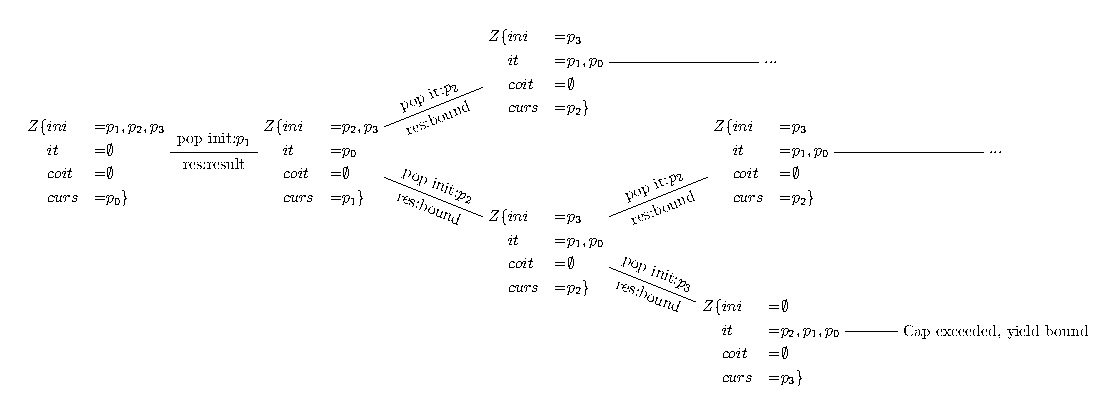
\includegraphics[width=\textwidth]{./imgs/cmds_tree.pdf}
\caption{\label{fig:cmds_tree}A tree of different evolution paths a
  zipper may undergo during between the calling of a process and the
  accumulated bound exceeding the cap. \(p_0\), \(p_4\), \(p_3\) and
  \(p_4\) are subprocesses. The values returned, the specific
  iteration subset data structure are not presented for brevity and to
  shift focus to the movement of the subprocesses within the
  zipper. Nodes in this tree that have two children correspond to the
  \hask{ItInit} constructor, nodes with one node correspond to the
  \hask{CmdIt} or \hask{CmdInit} constructor depending on which
  process set the process in the nex cursor is drawn from. When a
  concrete value is reached or the cap is exceeded the process stops
  and the free monad that wraps \hask{Cmds} takes the value
  \hask{Pure}.}
\end{figure}

\subsection{Resetting processes}
\label{sec:process_resetting}

In the subsection discussing the command functor we saw that it may
include a reset process. Why create a reset process when reusing the
initial process would reset the computation just as well? In any case
a reset moves all the init parts of the elements of iteration set as
well as the coiterations into the init set of the zipper. But in what
order? From previous runs it is often apparent that some execution
strategies are more likely to lead to a quick result than others. For
example, under the assumption that processes change their values less
often than they maintain them, while computing a logical AND operation
(\(\land\)) we likely want to start the computation from processes
that previously yielded \hask{False}.

To accommodate this, the \hask{Cmds} functor (introduced in section
\ref{sec:cmds_functor}) can yield a reset point. While running a
process we maintain in the lexical scope of the mealy arrows
computation the latest reset process to switch to when the
\hyperref[sec:epochs_coepochs]{epoch/coepoch} comparison requires as
much. When generating a \hask{Cmds} functor, the operator has the
option to implement the \hask{bgsReset} that resets a running zipper
that is at an arbitrary state. The signature and default
implementation are below:

\begin{haskellcode}
bgsReset :: ZipState w a -> ZipState w a
bgsReset bgs =
  mkGgState
  $ bgsInits bgs
  ++ (snd <$> toList (bgsIts bgs))
  ++ (snd <$> bgsCoits bgs)
\end{haskellcode}

\section{General operators}
\label{sec:antisthenis_ops}

While describing the core concepts of Antisthenis we often dealt with
functionality that is operator specific. Indeed, a large part of
Antisthenis depends on operator specific logic. We define operators at
three levels, each refining the previous. The lower levels are
parameterized by the higher ones.

The lowest level is reified as an uninhabited type, or tag, witnessing
the implementation of \hask{ZipperParams}. This implementation would
be build a workable Antisthenis type. The operator specific types are
presented in listing \ref{lst:zipper_params}. We have implemented a few types
in antisthenis to cover the needs of FluiDB (see listing
\ref{lst:tag_types}).


\begin{code}
\begin{haskellcode}
-- Result types
class BndRParams w where
  -- The result type when the value is non-computable
  type ZErr w :: *
  -- The partial result.
  type ZBnd w :: *
  -- The full result
  type ZRes w :: *

-- Zipper internal types
class BndRParams w => ZipperParams w where
  -- The type of the process cap
  type ZCap w :: *
  -- The type of the process epoch
  type ZEpoch w :: *
  -- The type of the coepoch
  type ZCoEpoch w :: *
  -- The type of the iteration set
  type ZItAssoc w :: * -> *
  -- The type of the partial result
  type ZPartialRes w :: *
\end{haskellcode}
  \caption{\label{lst:zipper_params}Operator specific types that need
    to be impolemented by every operator.}
\end{code}

\begin{code}
\begin{haskellcode}
-- The witness type for the sum operator
data SumTag p
-- The witness type for the minimum operator
data MinTag p
-- The witness type for multiplication
data MulTag p
-- The witness type for logical And/Or
data BoolTag op
\end{haskellcode}
  \caption{\label{lst:tag_types}Tags are phantom types that define the
    antisthenis operations. The tags themselves may be parameterized
    using type parameter \hask{p}. For the needs of FluiDB we define
    operations for addition, subtraction, multiplication and boolean
    operations.}
\end{code}

The parametric part of the tags, especially for \hask{SumTag} and
\hask{MinTag}, is due to the fact that we want to be able to further
parameterize them for concrete cost calculation (using sum and min
operators normally) and for stochastic cost calculation (see section
on \ref{sec:historical_cost} historical cost). These two both utilize
minimums and sums, but they use different types for return values as
well as caps/bounds and epochs/coepochs.

Since all types and implementations can be derived from the
\hask{ZipperParams} type \hask{w}, the Antisthenis process creation
function can be as simple as in listing \ref{lst:mkproc}, where
\hask{mkProc} combines a list of subprocesses into a parent process
that evaluates the operator described by the tag \hask{w} without
requiring any further information.

\begin{code}
\begin{haskellcode}
mkProc
  :: (Monad m,ZipperParams w,Eq (ZCoEpoch w)) => [ArrProc w m] -> ArrProc w m
\end{haskellcode}
  \caption{\label{lst:mkproc}The type \hask{w} fully defines the
    operator so combining subprocesses into a process is unumbiguous.}
\end{code}

\subsubsection{Compatibility  between heterogeneous processes}

The astute reader has likely noticed that \hask{w} is the parameter of
both the subprocesses and the process. The reason is that a process
expects to see a specific type of coepoch and bound returned by its
subprocesses, while the subprocess must be able to deal with the epoch
and cap that the parent process is defined for. To do that we avoid
defining an \(N \times N\) correspondence between all the epochs, but
rather we define ad hoc a record that facilitates the conversion, the
type of which is presented in listing \ref{lst:conv_def}. This way we
can compartmentalize the translation among operators from the internal
logic of the operators.

\begin{code}
\begin{haskellcode}
data Conv w w' =
  Conv
  { convEpoch :: ZEpoch w' -> ZEpoch w
   ,convCoEpoch :: ZCoEpoch w -> ZCoEpoch w'
   ,convCap :: ZCap w' -> ZCap w
   ,convRes :: ZRes w -> ZRes w'
   ,convBnd :: ZBnd w -> ZBnd w'
   ,convErr :: ZErr w -> ZErr w'
  }
convArrProc :: Monad m => Conv w w' -> ArrProc w m -> ArrProc w' m
\end{haskellcode}
  \caption{\label{lst:conv_def}An object of type \hask{Conv w w'} can
    act as an interface between parent processes of type \hask{w} to
    subprocesses of type \hask{w'}.}
\end{code}


\subsection{Basic cost operators}

General cost refers to minimum and sum operators with some special
semantics:

\begin{itemize}
\item Non-computable values are larger than any value from the
  perspective of minimum.
\item All values are positive (therefore all values are implicitly
  bounded by \([0 - \epsilon)\)
\end{itemize}

The minimum operation computes the minimum of the argument
operations.

\begin{itemize}
\item Iteration data structure of the minimum is a heap-like structure
  where we can peek at the top element and look into the secondary one
  and it also contains the value derived from the s encountered.
\item Zipper cursor always contains the most promising.
\end{itemize}

\subsubsection{Sum}

We do not implement a general sum operator but rather a sum operator
that assumes the properties of query costs as the values it deals
with. The sum is probably the simplest operator implemented. The
adding zipper evaluates each initial subprocess under a cap
\(c_{subproc}\) that is

\[
c_{subproc} := c_{parent} - r_{partial}
\]

where \(r_{partial}\) is the partial result omitting the cursor, ie
the current subprocess and \(c_{parent}\) is the cap that the parent
process is operating under. If the parent cap is \hask{ForceResult} all
arguments are also evaluated under \hask{ForceResult}. Of course if
\(c_{parent} > r_{partial} + b_{cursor}\) then \(r_{partial} +
b_{curopr}\) is returned as the result bound.

\subsubsection{Multiplication}

Multiplication is not used by FluiDB but is implemented in Antisthenis
nonetheless as a reference because it is fairly simple and yet it
implements exploits many of the features of Antisthenis. The
multiplication goes through all the initial subprocesses capping them
at zero until one of them returns a concrete result of zero in which
case the final result is also zero. Because a bound returned by a
process is strictly greater than the cap all the iterating results are
guaranteed to not be absorbing elements. Then multiplication proceeds
in the same way as addition does only multiplying instead of adding:

\[
c_{subproc} := c_{parent} / r_{partial}
\]

\subsubsection{Minimum}

Much like the sum operator, the minimum operator implementation also
assumes that it is manipulating cost types, and it is used in
conjunction with the sum operator to define our cost evaluations. The
operation of the minimum Antisthenis operator depends heavily upon the
iterator set which has the interface of a heap. The zipper evolution
stategy is described by the pseudo-python code in listing
\ref{lst:min_zipper_evolution}

\begin{code}
\begin{pycode}
def exceeds_cap(cap, zipper):
    return zipper.iter_procs.min().bound > conf.cap \
        and zipper.coiter_procs.min().result > conf.cap \


def minimum_zipper_evolution(conf,zipper):
    # Run each initial process with a zero bound
    while len(zipper.initial_procs) > 0:
        zipper.inter_procs.push(cursor)
        zipper.cursor = zipper.initial_procs.pop()
        res,nxt_proc = zipper.cursor.run(conf{cap = 0})
        # We cant hope to get a cost lower than zero
        if res == BndRes(0):
            # Until the epoch is updated
            return BndRes(0)

        # Push it to the correct iter set.
        if res.is_bound():
            zipper.iter_procs.push(res,nxt_proc)
        else:
            zipper.coiter_procs.push(res,nxt_proc)

    # Run the iterating processes
    while True:
        # If the result is better than the best iteration, it's the final result
        if zipper.coiter_procs.min().result < zipper.iter_procs.min().bound:
            return BndRes(zipper.coiter_procs.min().result)

        # If there are two iter processes
        if not exceeds_cap(conf.cap,zipper):
            # Run the best iterating process until it exceeds the
            # second best iterating process or the final result
            cap = min(zipper.iter_procs.second_min().bound,
                      zipper.coiter_procs.min().result)
            res,nxt =  zipper.iter_procs.min().run(conf{cap = cap})
            # Push it to the correct iter set.
            if res.is_bound():
                zipper.iter_procs.push(res,nxt_proc)
            else:
                zipper.coiter_procs.push(res,nxt_proc)
        else:
            conf = yield zipper.iter_procs.second_min().bound
\end{pycode}
  \caption{\label{lst:min_zipper_evolution}Pseudocode for the
    algorithm of evaluating a process up to a threshold defined by the
    cap. For brevity and to avoid too much unnecessary detail we omit
    sanity checks and the reset handling code.}
\end{code}

\subsubsection{Boolean conjunctions and disjunctions}

Antisthenis implements operators for boolean conjunction and
disjunction in order to be able to answer the question of whether a
node is materializable in the presence of a specific inventory of
materialized nodes. Booleans are different to the other operations in
how they handle caps. Boolean \(\land\) and \(\lor\) do not use the
same type for caps and bounds as for results. Instead the bound is a
two dimensional value that represents the minimum number of steps
required to arrive to each possible value (\hask{True} or
\hask{False}).

To efficiently evaluate boolean algebra expressions we make look for
absorbing elements, which this time demonstrates how absorbing
elements can be exploited to prune the expression tree, consider the
problem of evaluating a Boolean expression \(A \land B \land C\) where
\(A\), \(B\) and \(C\) are subexpressions. Obviously if any of the
expressions \(A\),\(B\) or \(C\) evaluates be \hask{False} the entire
expression would consequently evaluate to \hask{False} as well as
\hask{False} is the absorbing element for the group of booleans over
\(\land\). Furthermore without taking into account the structure of
each of the subexpressions \(A\), \(B\) and \(C\) we can tell that the
amount of work for evalutating it depends on the result. If the result
of this expression is \hask{False} then the best case scenario in
terms of amount of work we would need to do is for A to be the
expression \hask{False}. In this case we would be able to evaluate the
expression with just one dereference. If the result is \hask{True}
then the best case scenario is for \(A\), \(B\) and \(C\) to all be
\hask{True} and we would be able to come to a result with three
dereference steps.

Consider the expression

\[
X := (A_1 \lor A_2 \lor A_3) \land (B_1 \lor B_2) \land (C_1 \lor C_2 \lor C_3)
\]

Where \(A_i\), \(B_i\) and \(C_i\) are expressions. How would we
navigate this expression to minimize the number of operations?  We
could completely expand each term and hope that we are lucky, and we
encounter absorbing elements early on. As explained in the
introduction, especially for terms automatically generated this
strategy is unlikely to be efficient.

Instead, at each expansion we count the minimum number of steps
required for each value. In the above example the best case scenario
if the value of \(X\) is \hask{False} is \(B_1 = False\) and
\(B_2 = False\), in which case the expression is evaluated in a
minimum of 4 steps:

\begin{itemize}
\item Evaluate \(B_1 = False\) in a single step
\item Evaluate \(B_2 = False\) in a single step
\item Evaluate the subexpression \(False \lor False\)
\item Evaluate \(X = (...) \land False \land (...)\)
\end{itemize}

For a value of \hask{True} it is 7:

\begin{itemize}
\item Evaluate \(A_i = True\) in a single step for any \(i\)
\item Evaluate the subexpression \(True \lor ...\)
\item Evaluate \(B_i = True\) in a single step for any \(i\)
\item Evaluate the subexpression \(True \lor ...\)
\item Evaluate \(C_i = True\) in a single step for any \(i\)
\item Evaluate the subexpression \(True \lor ...\)
\item Evaluate \(X = True \land True \land True\)
\end{itemize}

A boolean expression in Antisthenis, then, takes the bound value of
the minimum cost for trues and falses. If this expression were
evaluated with a cap of \(\{True: 6, False: \infty \}\) it would
return a bound of value \(\{True: 7, False: 4 \}\). In plain english
this means "try to evaluate this if your other options are more
expensive than 7 steps for \hask{True} and 4 for \hask{False}". It
should be seen as a metric for the size of the tree.

To demonstrate the derivation of caps we present the following
expression:

\[
X = X_1 \land X_2 \land X_3
\]

Any of the \(X_i\) terms has a minimum bound of
\(\{True: 1, False: 1 \}\). Since the absorbin element for \(\land\)
is \hask{False} expanding any of the \(X_i\) terms is bounded by
\(\{True: \infty, False: 1 \}\) bacause so an expansion of

\[
X_1 = A_1 \lor A_2
\]

Would cause the subprocess to immediately yield
\(\{True: 2, False: 3 \}\) passing control to the parent
process. Thus, a symmetrically growing tree would be traversed in a
breadth first fashion and any asymmetries would cause Antisthenis to
try to greedily exploit the smaller parts of the tree.

Antisthenis has a different regime for comparing caps and between a
cap and a bound. We consider that a bound exceeds a cap when either
the steps to a true final value or the steps to a false final value
exceed the corresponding cap. However when it comes to comparing
bounds we consider the better bound to be the more optimistic one.

\begin{align*}
b_1 <_{bnd} b_2 := \min(T(b_1),F(b_1)) < \min(T(b_2),F(b_2))
c <_{cap} b := T(c) < b \land F(c) < F(b).
\end{align*}

where for \(x\) being a bound or a cap, \(T(x)\) is the minimum number
of dereferences assuming the final value is \hask{True} and \(F(x)\)
is the minimum number of dereference values assuming the final value
is \hask{False}.




\section{Node machines}

A referrable machine is a process with a name that can be referenced
by more than one other processes. In FluiDB a machine name corresponds
to a graph node since the antisthenis infrastructure is utilized to
provide incremental computation of properties on nodes
(materializability, cost, stochastic cost, etc are described in
separate sections). In this section we look into the the layer of
antisthenis that takes into account the dynamics of referrable
machines.

\subsection{Antisthenis machine tape}

The machine tape is a dynamic directory that maps nodes to
machines. The meaning of a node is dependent on the implementation, in
the context of FluiDB nodes in this context correspond to the FluiDB
internal graph nodes. The machine tape is part of the computation
context and is updated by new and temporary values of machines (see
section \ref{sec:cyclical_machines} on cyclic machines).

Not all processes involved in a computation are involved in the
machine tape. Each machine in the tape is composed by a hierarchy of
machines that are inaccessible from outside. In fact a machine is
discriminated from a process solely by virtue of the fact that it can
be referenced via the tape. A parallel might be drawn between machines
as being like C++ lvalues in that they are referable by an address,
and processes being like rvalues in that they are still values but
they are completely nameless. Furthermore, as the astute reader will
have noticed, it may not be clear in every context when a process
stops being itself. Remember that a process is fundamentally a mealy
arrow (introduced in section \ref{sec:mealy_arrows}) which once
evaluated returns a new mealy arrow, the next version of
itself. Self-sameness is much more concrete in the case of machines,
as machines are always referred by exactly one slot in the tape.

Since machines are referable by different other processes it means
that, we need to be carful that more than one process do not own their
own diverging copy of the same machine, essentially treating it as a
process. To avoid this issue, processes referring to machines do so
indirectly via a \textbf{machine wrapper process}. A machine wrapper is a
process that does the exact same thing every time it is evaluated:

\begin{itemize}
\item it looks up a name in the tape
\item it temporarily replaces it with a cyclical machine (see section
  \ref{sec:cyclical_machines})
\end{itemize}

The machine tape evolves externally to each individual process and
each process evolves within the tape itself. We implement it inside a
state monad in the underlying Kleisli arrow. Thereby a recursive
reference is formed between the tape and the machine.
\subsection{Process stack}
\label{sec:process_stack}
Before we go further with the details of how exactly named machines
are handled, it is important to make the discrimination between a
process and a computation. In the context of Antisthenis a process, or
in case it is named a machine, is the mealy machine that evolves
during evaluation and survives between evaluations. On the other hand
a computation is the part of the evaluation itself that refers to the
particular machine. At the risk of getting too philosophical, a
computation is the \textbf{relation} between the process and the value
produced, regardless of whether that value is an actual result, a
bound for a potential result or a witness to the non-computability of
the result.

With this distinction in mind we introduce the notion of a process
stack which is similar to the notion of a call stack in any
programming language. The process stack contains all processes that
have live computation. When a process is called, it is pushed to the
process stack and when a result is returned it is popped from the
process stack. The process stack is completely ephemeral, acyclic and
should be completely empty between computations. In this sense it is
part of the \textbf{computation context}, the sum of effects that
affect each computation separately. The computation context may be
implicit (like in the case of the process stack as we will see when
discussing \hyperref[sec:cyclical_machines]{cyclical machines}) or
explicit in the process' underlying Kleisli arrow.

\subsection{Cyclical machines}
\label{sec:cyclical_machines}

By virtue of machines being referable by arbitrary other machines, it
is possible, and certain in the case of FluiDB, that the Antisthenis
machines will form referential cycles. Such cycles in most
computational frameworks, especially ones that deploy a non-lazy order
of computation, will cause the computation to either fail or to
not-terminate. Antisthenis is explicitly designed around allowing the
computation to handle such self-referential cases.

We already discussed in a previous section that machines are stored in
data structure called a tape that allows us to reference them, and
that in the period from the time a value is requested of a machine and
the time a value (including an error or a value bound) the machine is
said to be in the computational stack (introducted in section
\ref{sec:process_stack}). During its residence in the stack a machine is
in a state where it is unable to produce a value. A cycle occurs when
a machine is referenced while in the computational stack.

We make the problem concrete with an example based on the graph in
figure \ref{fig:recur_package}. A naive approach of dealing with
recursive calls is demonstrated in figure \ref{subfig:comp_d_naive} where
naive-Antisthenis looks for cycles by throwing errors (\(\bot\)) when
encountering a node that is already in the computational
stack. Evaluating node \(A\) Antisthenis first node \(B\) to 10. It
then tries to evaluate node \(C\) which redirects back to \(A\). \(C\)
can therefore not yield a value and returns an error \(\bot\). Then,
without changing any of the parameters the user tries to evaluate
\(D\). Looking at the graph it is clear that \(D\) should in sequence
evaluate to 15, as demonstrated by the evaluation process in figure
\ref{fig:comp_d_smart} (the reader is reminded that based on the assumption
that all values refer to query evaluation costs we have asserted that
\(min[a,\bot] \equiv a\)).


\newcommand{\newl}{\\ \ }
\newcommand{\ev}{\!\!\Rightarrow\!}
\newcommand{\comp}[3]{%
  \left.\begin{array}{l}
comp[#2] \!: \\
\ #3 \\
\end{array}\!\right] \ev #1%
}
\newcommand{\colw}{5cm}
\begin{figure}[p]
  \begin{subfigure}{0.9\linewidth}
    \begin{tikzdiagram}
      \tikzset{f /.tip = {Stealth[scale=2]}}
    \tikzstyle{every node}=[ellipse,draw];
    \node (a) at (0,0) {$A:=min[B,C]$};
    \node (b) [below left=1cm and 0.5cm of a] {$B:=10$}
      edge [f-] (a);
    \node (d) [right=of a] {$D:=C+2$};
    \node (c) [below right=1cm and 0.5cm of a] {$C:=A+3$}
      edge [f-] [bend right=15] (a)
      edge [-f] [bend left=15] (a)
      edge [f-] (d);
    \end{tikzdiagram}
    \caption{\label{fig:recur_package}A recursive cost graph.}
  \end{subfigure}
  \begin{subfigure}{0.9\linewidth}
    \[
      \comp{\bot}{A}{
        comp[B] \ev 10 \\
        \comp{\bot}{C}{comp[A] \ev \bot}}
    \]
    \caption{\label{subfig:comp_a}Computation for \(A\)}
  \end{subfigure}

  \begin{subfigure}{0.4\linewidth}
    \[
      \comp{\bot}{D}{comp[C] \ev \bot}pp
    \]
    \caption{\label{subfig:comp_d_naive}Naive computation for \(D\)}
  \end{subfigure}
  \begin{subfigure}{0.4\linewidth}
    \[
    \comp{10}{D}{
      \comp{10}{C}{
        \comp{10}{A}{
          comp[B] \ev 10 \\
          \ comp[C] \ev \bot}}}
  \]
  \caption{\label{subfig:comp_d_smart}Computation for \(D\)}
  \end{subfigure}
\caption{\label{fig:correct} Node C is recomputed
 because the \(\bot\) value is predicated on \(A\) being in the computation stack.}
\end{figure}

The root of the problem in the naive case is that the process stack is
an ephemeral property and yet it affects the return values that are
non-ephemeral. The only solution for this is to lift information about
the cycles to the non-ephemeral plane that survives the
computation. Indeed, what is needed is for values that are deemed
non-computable to \emph{reset} when accessed with a different stack. In
other words the value of \(\bot\) for \(C\) is \emph{predicated} on the
process stack containing \(A\), or \(A\) being otherwise
non-computable. Coepochs fill the bill precisely. We extend the coepoch
to include, along with the parameter versions used to derive a
particular result, also a set of machines that need to be
non-computable in order for the value to be valid.

To accomplish this when a machine is looked up, before being evaluated
it is removed from the tape and in its place a \textbf{cyclic machine}
is placed. This machine always returns the same \(\bot\) result that
indicates that the value is non-computable and sets to the coepoch
that it is itself not computable. When the original machine comes up
with a value it replaces the cyclic machine again and the coepoch is
sensored. This way whenever any machine tries to evaluate another
non-computable machine it finds a cyclic machine which handles the
situation automatically. Upon evaluating the cyclic machine, the
coepoch of the caller is infected with the predicate that the cyclic
machine must be \(\bot\). Pseudo-python algorithm in listing
\ref{lst:algo_create_predicates}.

\begin{code}
\begin{pycode}
def cycle_machine(node):
    # Return a process that returns non-comp and a predicate nofifying
    # that it is itself not computable.
    class CycleProc:
        def run(conf):
           return (lookup_node(node),non_comp,Coepoch(predicates=[node]))

    return CycleProc()

def run_submachine(node,conf):
    # Replace the real process with a dummy cycle process.
    p = lookup_node(node)
    insert_node(node,cycle_machine(node))
    nxt,res,coepoch = p.run(conf)
    insert_node(node,nxt)
    # Censor the current node from the predicates. If the result is
    # computable then the predicate is already falsified, if not it is
    # confirmed.
    return (nxt,res,coepoch{predicates=coepoch.predicates.delete(node)})
\end{pycode}
  \caption{\label{lst:algo_create_predicates}The algorithm for
    creating predicates.}
\end{code}

At the end of the computation Antisthenis goes through all the
non-computable predicates and asserts that they are indeed
non-computable. The ones that turn out not to be non-computable are
collected and set as \emph{copredicates} in the epoch. The node is
then reevaluated with the new epoch. Due to the incremental nature of
Antisthenis only the parts of the graph that are dependent on the
predicates are reevaluated. The process is described in listing
\ref{lst:algo_handle_prediates}

\begin{code}
\begin{pycode}
def safe_run(n,conf):
    # To check if new copredicates were added
    initial_copred_num = len(conf.copredicates)
    # Run the process
    coepoch,res,coit_p = lookup_node(n).run(conf)
    # Remember: machines censor their own reference from the predicate
    # and no predicates.
    assert n not in coepoch.predicates
    assert len(intersection(conf.epoch.predicates,coepoch.predicates)) == 0
    # For efficiency any result we find we register all resutls we
    # find that may be encountered later as predicates.
    conf.copredicates.push(n)
    # For each non computable predicate
    for noncomp_node in coepoch.predicates:
        # Run the predicate to check if indeed it is non-computable
        res = safe_run(lookup_node(noncomp_node), conf)
        if is_computable(res):
            # If it is actually computable then register it a copredicate.
            conf.copredicates.push(noncomp_node)

    if len(conf.copredicates) > initial_copred_num:
        return lookup_node(n).run(conf)
    else:
        return res
\end{pycode}
\caption{\label{lst:algo_handle_prediates}Algorithm for handling the predicates.}
\end{code}

Another way to look at predicates is as deferred parts of the coepoch,
to get the full coepoch we also need the coepochs of the
predicates. The copredicates then are a forcing mechanism where
Antisthenis assumes that some of deferred parts are actually
invalid. Antisthenis is lazy with these coepochs first and foremost
because it depends on it to handle cycles but also because coepochs
may be inhibited by absorbing elements, and it may not need to
evaluate them at all. But if a predicate survives both the process
stack based censoring that we just described and being inhibited by
the operators, Antisthenis has another trick up his sleeve: because it
has a completely relativistic view of values, where they are only
valid for particular epochs, the only requirement at every moment is
that the final result of the computation be correct. Furthermore, the
value depends on the machines in the predicate being
\(\bot\). Therefore, it is enough to check that they are indeed
\(\bot\) certifying the predicates. The predicates that are falsified
in this way are the ones for which there is no other option but to
force their value be taken into account via the epoch's copredicates.


\subsection{Calculating historical query costs}
\label{sec:historical_cost}

As we saw in section  on the query planner, the planner depends
on the cost of past nodes to make decisions about the overall
usefulness of a plan. A naive approach to this would be to just use
the normal min/sum operation set to calculate historical costs. As
explained in more detail in that chapter this approach is
problematic. We need a way of convincing Antisthenis to "look behind"
those materialized nodes a) without completely ignoring the
materialized nodes and b) by handling referential cycles more
gracefully than declaring nodes non-computable. For this reason we
develop the \emph{stochastic costs model}.

The correct way of calculating the expected cost of a node in the
future, which we very informally and heuristically attempt to
approximate, would be to instead of considering the cost of
materialized nodes to be zero, to calculate the likelihood that a
materialized node will still be materialized when we encounter it
again. This is related not only to an estimation of how many
page-writes separate the moment of cost estimation and the actual plan
the cost of which is being estimated, but also all the decisions that
the garbage collector will make in that time. After FluiDB's budget is
exhausted for the first time, for every page write there a page needs
to be garbage collected. We considered a couple of options for
stochastically modelling the behavior of the GC like assuming that it
chooses random pages or random tables, but we could find none that was
useful and computationally viable.

For this reason we decided to follow a pragmatic approach to the
problem and simply assume that for every materialized node there is a
constant probability that it will not still be materialized when we
need it, scaling the cost by that factor to get the stochastic
cost. Furthermore, under this regime, Antisthenis would encounter many
more cycles, rendering virtually all machines non-computable. For that
reason we make all values semi computable by introducing a \([0,1]\)
scale where 0 would mean that the value is fully computable and 1
would mean that the value is completely non-computable.

Fortunately this change does not require a complete overhaul of the
operator implementations, only the definition of more complex types
for cap, bound and result values. Particularly, we qualify each value
with two numbers:

\begin{itemize}
\item the materialized nodes encountered
\item a quantification of the non-computability of the value
\end{itemize}

Some care needs to be taken so that the values remain independent of
the root of the computation.

The cap (listing \ref{lst:def_histcap}) is only qualified by the number of
machines corresponding to materialized nodes that are currently in the
computation stack, i.e. machines that would have otherwise yielded
zero cost.

\begin{code}
\begin{haskellcode}
data HistCap a =
  HistCap
  { hcMatsEncountered :: Int
   ,hcValCap :: Min a
   ,hcNonCompTolerance :: Double
  }
\end{haskellcode}
  \caption{\label{lst:def_histcap}Definition of the type used for
    capping the cost of historical queries.}
\end{code}

The bounds and results are augmented by two new dimensions (listing
\ref{lst:def_histres}):

\begin{itemize}
\item The \([0,1]\) computability metric
\item The maximum chain of materialized nodes encountered.
\end{itemize}

And the comparison between bounds and caps is presented in listing
\ref{lst:hist_compare}.

\begin{code}
\begin{haskellcode}
data HistRes a =
  HistRes
  { hrComp :: Double  -- [0,1] computability metric.
   ,hrMaxMatTrail :: Int -- Maximum trail of materialized nodes
                         -- encountered.
   ,hrRes :: a
  }
\end{haskellcode}
  \caption{\label{lst:def_histres}Definition of the type used for both
    bounds and results of historical queries.}
\end{code}


\begin{code}
\begin{haskellcode}
-- | We prefer "more computable" results than "less computable" so we
-- scale the actual result by the computability. We also define a
-- computability threshold under which we consinder the value always
-- >.
compare :: HistRes a -> HistRes a -> Comparison
compare (HistRes c1 t1 r1) (HistRes c2 t2 r2) =
  if
    | c1 > thr && c2 > thr -> compare (scale c1 r1) (scale c2 r2)
    | c1 > thr             -> GT
    | c2 > thr             -> LT
    | otherwise            -> compare a b
  where
    thr = 0.7

-- There are no circumstances under which we are going to choose a
-- value that has come through more materialized nodes. The scaling
-- will have damped it enough.
instance Ord a => Ord (Cert a) where
  compare (Cert _ a') (Cert _ b') = compare a' b'

extExceedsCap _ HistCap {..} HistRes {..} =
  maybe False (hrRes >) (unMin hcValCap)
  || hrMaxMatTrail bnd > (maxMatTrail - hcMatsEncountered)
  || hrComp bnd > hcNonCompTolerance
  where
    maxMatTrail = 5 -- actually this is part of a global config.
\end{haskellcode}
\caption{\label{lst:hist_compare}Comparison between bounds and
  between bound and cap are different. Between bounds we need to
  account for the computability metric. The cap on the other hand
  defines a three-dimensional bound () that the bound must fall
  within in order to not exceed it.}
\end{code}

\section{Conclusion}

In this chapter we described in detail the incremental evaluation
system we developed for FluiDB that we call Antisthenis. The main
goals of Antisthenis are to compute incrementally, to gracefully
handle computational cycles and to order the operations in an operator
specific way such that the overall computation finishes as soon as
possible.

There are two major shortcomongs of Antisthenis:

\begin{itemize}
\item Extending it to new operators and even using the existing operators
involves a lot of boilerplate. This is an immediate effect of the
current version of Antishtenis being highly specific to the FluiDB
planer.
\item Our current implementation relies heavily on the higher order
functional capabilities of haskell that are efficient for what they
are, but they stress the garbage collector and are hard for GHC to
optimize.
\end{itemize}

Both of these could be mitigated in a future version of Antisthenis
that would be detached from FluiDB and that would replace the
Antisthenis process with a more "traditional" data structure.

Further work could also be done to parallelize Antisthenis. Some
operations like \hask{min} rely on the operands being evaluated
serially to take advantage of early stopping but addition is much more
flexible with the order of evaluation. It is clear that parallelism
would also be implemented in an operator specific way.

%%% Local Variables:
%%% mode: latex
%%% TeX-master: "thesis"
%%% End:
